In this chapter we first provide an overview of traditional robot programming techniques and categorise them to identify common bottlenecks.
We discuss state-of-the-art techniques in manual (\sect{subsec:Manual Programming Systems}) and automatic (\sect{subsec:Automatic Programming Systems}) programming systems and their required end-user involvement in the programming process (\sect{sssec:End-User Involvement}).
We end this chapter by discussing common encountered issues and relations to this thesis (\sect{sota-discussions}).

\section{Introduction}
Robot Programming is the process of defining desired motions and associated skills of the robot that it may perform without human intervention.
Classical robot programming processes in the industry have task-specific definitions, which are generally robot-dependent, and require programming expertise.
Figure \ref{fig:Classical robot programming process} shows the classical robot programming process, consisting of at least four phases:
The initial definition of a resource-centered task and layout is followed by sequencing the workcell operations.
Once the process has been validated, the robot is programmed offline using one or more native robot programming languages, before it is pushed into production for regular execution.
The programmed robot can only be used for this specific task in this particular working environment.
If the task definition needs to be modified, the programming expert has to repeat the entire programming process to ensure a consistently valid execution in production.
Therefore, classical robot programming processes can be very time-consuming and cost intensive.

\begin{figure}[ht]
	\centering
	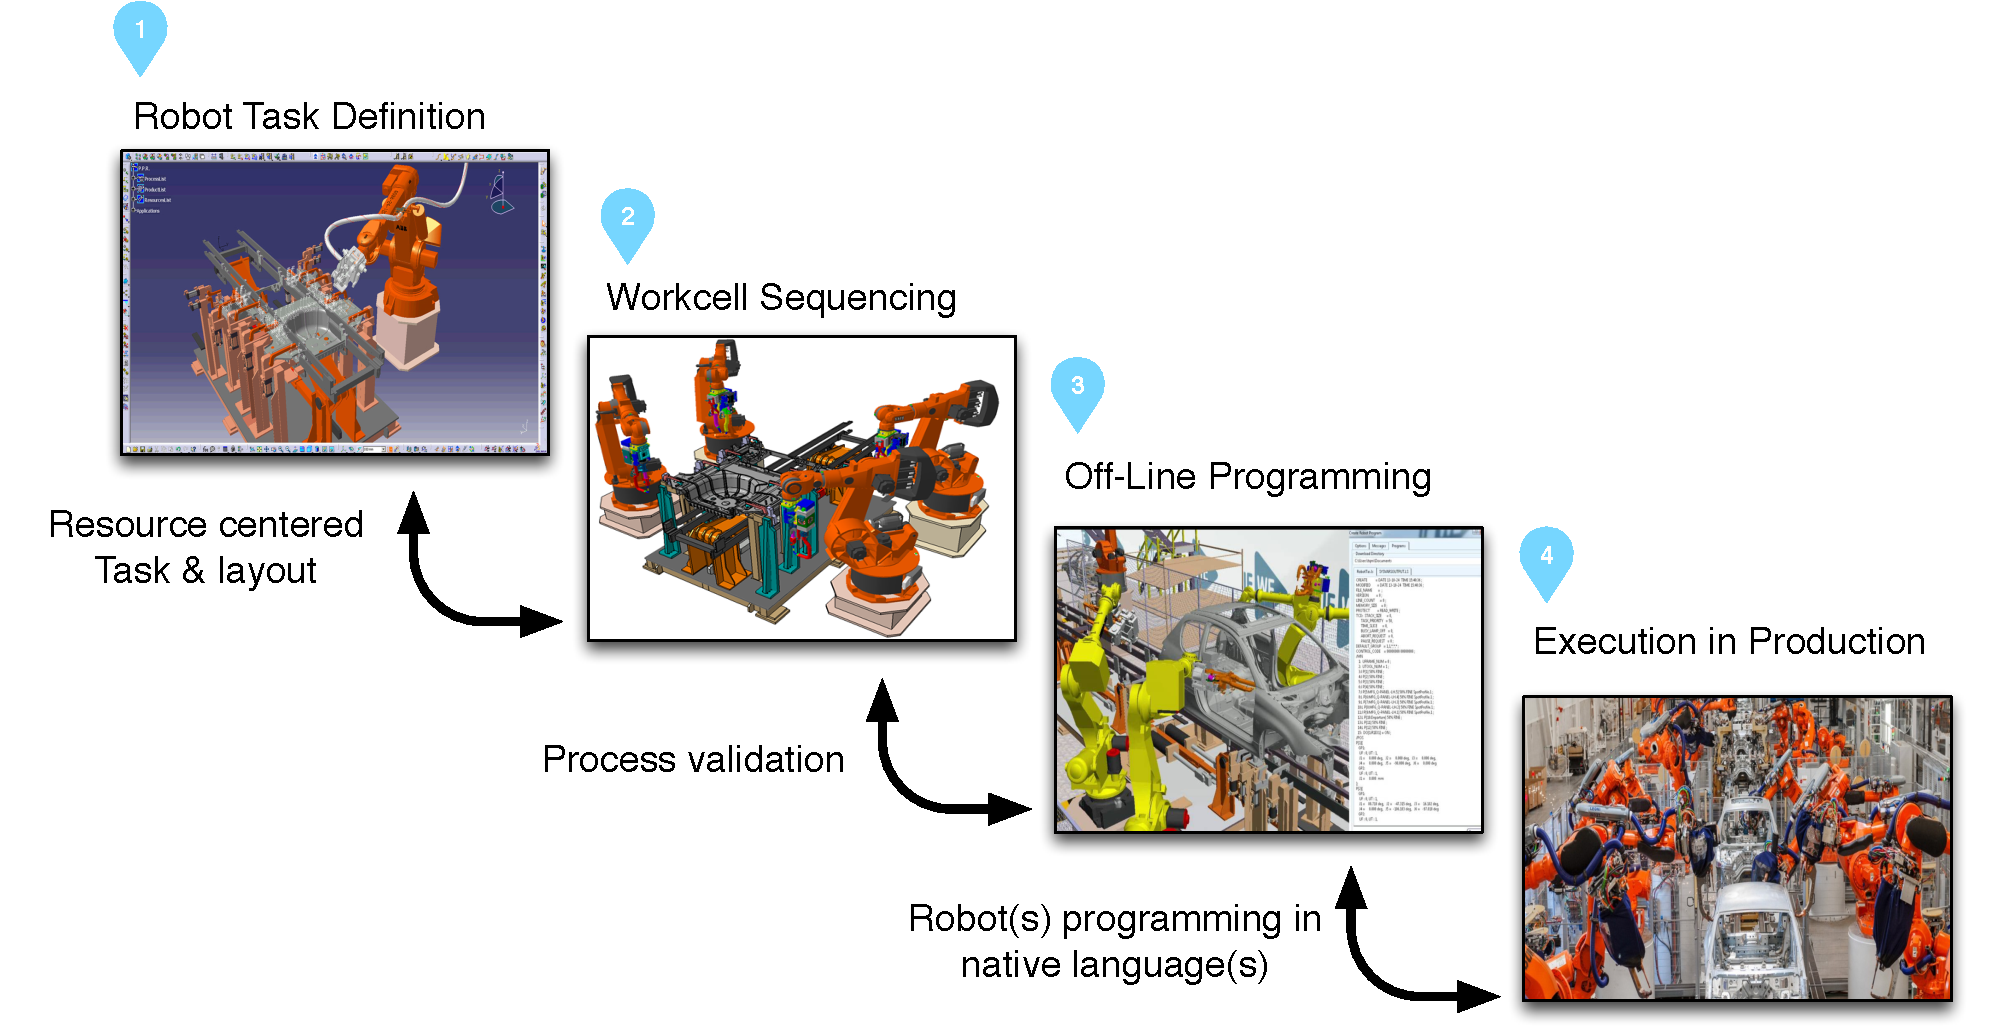
\includegraphics[width=\linewidth]{figures/manual-programming}
	\caption{Classical robot programming process}
	\label{fig:Classical robot programming process}
\end{figure}

In the past few decades, different robot programming techniques have been developed to facilitate this process. 
There are many ways to divide robot programming systems. 
\cite{lozano1983robot} divided them into three categories: 
guiding systems, where the robot's joint positions are sequentially recorded,
robot-level systems, where a programming language is used, and
task-level systems, where the task goal (\eg object positions) needs to be specified.
However, the range of programming systems was very limited at that time and examined only industrial robot programming systems.
Instead, \cite{Biggs2003} divided them into two main categories, distinguishing programming methods between systems for programmers and users:

\begin{itemize}
 \item {\textbf{Manual programming:} the user can directly control the robot's execution code, using a text-based or a graphical system.}
 \item {\textbf{Automatic programming:} the user does not need to write explicit code and the robot learns using a learning or an instructive system.}
\end{itemize}
% - also mention software architectures which are important for any robot programming systems

% \begin{figure}[ht]
% \centering
%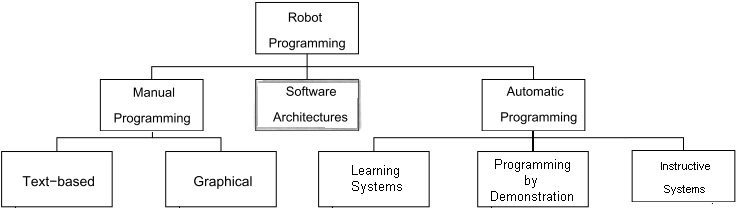
\includegraphics[width=\linewidth]{figures/Biggs2003-RobotProgramming-short}
% \caption{Robot programming categories to distinguish systems for users and programmers. (\cite{Biggs2003})}
% \label{fig:RobotProgrammingSystems}
%\end{figure} 

Inspired by these main categories, we created an overview of the main robot programming techniques that have been applied in most recent research (\fig{fig:RobotProgrammingOverview}).
Even though many state-of-the-art systems use a combination of techniques, such as Deep Reinforcement Learning (\cite{arulkumaran2017brief,mnih2015human}) or PbD for Reinforcement Learning (\cite{hester2017learning}), it makes sense to differentiate them by their key attributes, which we identified as follows: 
%control over the robot code, learning data, and end-user involvement.
\begin{itemize}
	\item \textbf{Control over the robot behaviour:} if the code created by the user directly encodes the robot's executed behaviour (manual vs automatic programming), and if created manually, how the code is generated (text-based vs visual programming)
	\item \textbf{Learning data:} for automated programming systems the robot learns from data, so we differentiate between the type of data used: if the data is biased or unbiased, if the teacher is involved in the learning process, how the data is acquired (provided by a teacher vs by self-exploration), and if it is labelled (supervised vs unsupervised learning) %(\eg positive vs negative examples, labelled)
	\item \textbf{End-user involvement:} the level that the end-user is involved in the programming process ranges from writing code manually, providing data or continuous feedback during the learning process to defining reward functions.
\end{itemize}

%From an end-user programming perspective, it is useful to assign different levels of teacher involvement in the programming process and an estimation of the programming time required.
In the following sections we will give a brief overview of the identified programming system categories by first distinguishing between the user's control over the robot behaviour, \ie manual (\sect{subsec:Manual Programming Systems}) and automatic (\sect{subsec:Automatic Programming Systems}) programming.
For manual programming, we compare text-based (\sect{sssec:Text-based Systems}) and graphical (\sect{sssec:Graphical systems}) systems.
For automatic programming, we differentiate between those that learn from unbiased and biased data, \ie machine learning systems (\sect{sssec:Learning Systems}) vs programming by demonstration (\sect{sssec:PbD}).
Finally, we will discuss different levels of end-user involvement %and their interaction modalities 
(\sect{sssec:End-User Involvement}) and conclude this chapter by discussing relations to this thesis (\sect{sota-discussions}).

%\begin{table}[ht]
%\begin{center}
%\begin{tabular}{r|c|c}
%Programming Techniques & by Exploration \newline (unguided) & by Demonstration \newline (guided)\\ \hline
%Classification & \checkmark & \checkmark \cite{saunders2006teaching,hovland1996skill,rybski1999interactive} \\
%Regression & \checkmark & \checkmark \cite{atkeson1997locally,pomerleau1991efficient} \\
%Reinforcement Learning & \checkmark & \checkmark (System models) \cite{atkeson1997robot,smart2002effective,abbeel2004apprenticeship}.\\
% Plans & \checkmark & \checkmark \cite{kuniyoshi1994learning,ekvall2008robot} \\
% \hline
%Human-Robot Interaction & & \\ \hline
% touch & \checkmark (learning by poking) & \checkmark \\
% vision & \checkmark & \checkmark \\ 
% voice & n/a & \checkmark (instructive, create sequence by voice) \\
%\end{tabular}
%\end{center}
%\label{tab:Programming Overview}
%\end{table}

\section{Manual Programming Systems}\label{subsec:Manual Programming Systems}
In manual programming systems, users have direct control over the robot code
for which they often require expert knowledge in a programming language. % and a good understanding of the program flow.
There exists a variety of tools to make programming, as well as testing and debugging, easier such as IDEs, spreadsheets or macros. 
There are two types of manual programming: text-based programming, where the code is written manually in a chosen programming language (\eg python, C++, java) and graphical programming, where the code structure is created with the help of a graphical interface (\eg flow-charts). 

\clearpage
\begin{sidewaysfigure}[!h]
	\centering
	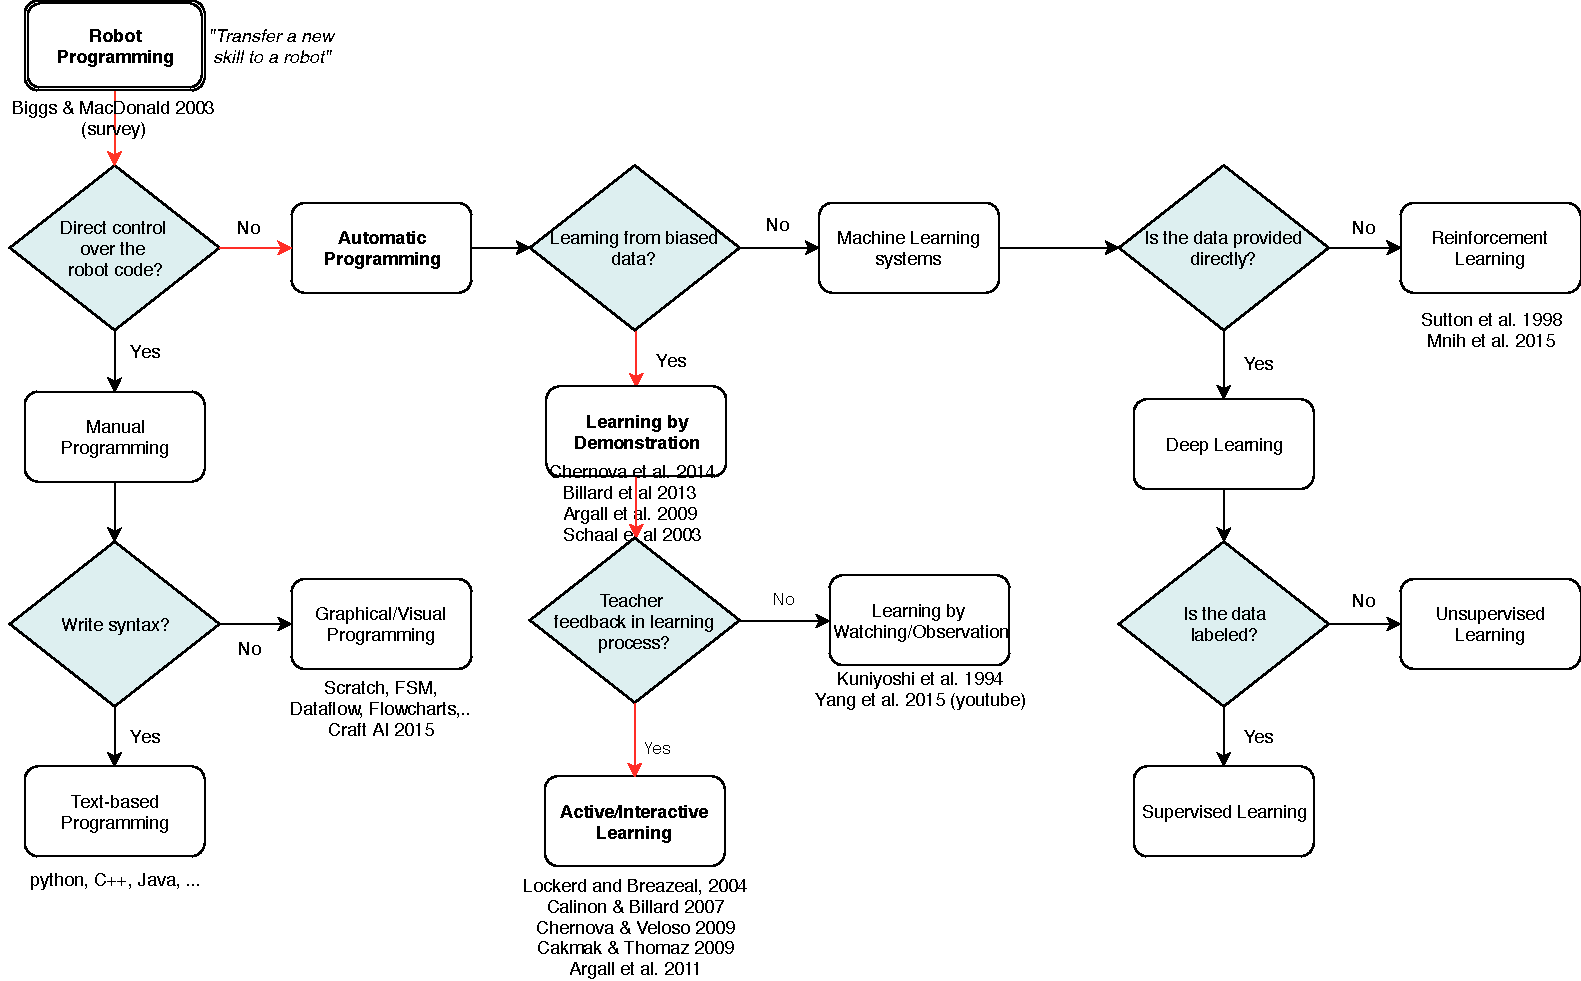
\includegraphics[width=0.95\linewidth]{figures/RobotProgrammingOverview}
	\caption{Overview of Robot Programming approaches based on control over robot behaviour code, type of learning data and how it is acquired and teacher feedback. Approaches are ranked by end-user involvement in the programming process as well as data and time required to learn a skill.}
	\label{fig:RobotProgrammingOverview}
\end{sidewaysfigure}
\clearpage


\subsection{Text-based Systems}\label{sssec:Text-based Systems}
Text-based systems are one of the most common methods and use a traditional programming approach. 
\cite{Biggs2003} differentiated between the type of programming language used:
The user programs in either controller-specific languages, where the machine language consists of simple commands specific to the robot (\eg the KUKA Robot Language (\cite{braumann2011parametric,muhe2010reverse}) shown in \fig{fig:Kuka}),
% RAPID a high-level programming language to control ABB robots
generic procedural languages, where multi-purpose languages such as C++ have been extended with classes to provide simple access to common robot specific functions ({\eg \cite{lego2003}}), or behaviour-based languages that specify how the robot should react to different conditions (\eg Haskell (\cite{hudak2002arrows})). 
There has been a trend to move from low-level command-based languages towards more intelligent programming systems (\eg IDEs) with high-level languages that provide more support to the user and reduce the programming workload.
However, text-based systems are more likely to be used by robot developers than end-users as they still require trained users with programming knowledge.

\subsection{Graphical Systems}\label{sssec:Graphical systems}
Graphical or icon-based systems use a graph, flow-chart or diagram view where users manually specify actions and program flow.
The graphical icons correspond directly to predefined program statements.
\cite{lego2003} and \cite{bischoff2002morpha} produced graphical systems using a flow-chart approach, where the robot's behaviour can be configured by arranging low-level actions in a sequence (\fig{fig:lego-mindstorm}).
Similarly, Scratch (\cite{majed2014learn}) is a block-based visual programming language to allow children with no programming experience to learn development in an intuitive way for animations and interactive applications (\fig{fig:scratch-interface}).
Blockly (\cite{fraser2013blockly}) is a framework for building visual programming languages and has been used for programming mobile manipulator robots with a drag-and-drop interface as a high-level programming component (\cite{huang2016design}).
While the user does not have to write code explicitly, they still have to manually sequence the components for the robot's behaviour.
Thus, graphical systems still require some amount of programming effort and expertise to create the logical consistency of the robot program.
%They are typically easy to use and generally used for robot applications rather than system programming. 
\section{Automatic Programming Systems}\label{subsec:Automatic Programming Systems}
Automatic programming systems relate to robots that can generate their behaviour from data provided as input to the system.
Unlike manual programming, the end-user does not need to write or sequence robot code and does not have direct control over the robot's executed behaviour.
%\subsection{Deriving a policy}\label{subsec:Deriving a policy}
%Our focus is on the former, learning low-level trajectories that can be generalised.
%The latter will then be taken over by automated planning techniques.
The problem of learning a behaviour or \textit{skill} can be considered as learning a function, referred to as a \textit{policy}, that maps a world state to an action.
In real-world applications, states can only be partially observed due to restricted sensor availability.
Hence, we assume that the robot learner has access to the observed state $Z$ instead.
A policy is a state-action mapping $\pi : Z \rightarrow A$ that allows the robot to select actions from an action domain $A$, given observations of the observed world state $Z$.
States can either be represented in a discrete way (\eg \textit{`object on the table'} or \textit{`robot holding object'}) or in a continuous way (\eg $(x,y,z)$ coordinates of the object position)).
Table \ref{tab:representations} shows examples of the different representations for common state observations (\eg object position, orientation, colour, spatial relation).

\begin{table}[ht]
	\centering
	\caption{State representations: continuous vs discrete}
	\label{tab:representations}
	\begin{tabular}{r|ll}
		& Continuous representation & Discrete representation\\ \hline
		Position & $(x,y,z)$ coordinates & table \\
		Orientation & ($\theta_x,\theta_y,\theta_z$) angles & straight/upright \\
		Colour & $(r,g,b)$ values & red, yellow, green\\
		Spatial relation & $(x,y,z)$ distance vector & left/right/front/behind of 
	\end{tabular}
\end{table}

%Once the training data has been acquired, the robot learner needs to derive a policy $\pi : Z \rightarrow A$, 
There are different techniques to derive the policy that represents the desired behaviour from the observed state.
The most efficient policy derivation techniques approximate the state-action mapping from as few training data as possible.
\cite{chernova2014robot} give an overview of state-of-the-art techniques for robots learning from human teachers and differentiate between policies that represent low-level \textit{motions} and high-level \textit{tasks} which use these motions. 
%In the following we will give an overview of both techniques.

\begin{figure}[!h]
	\centering
	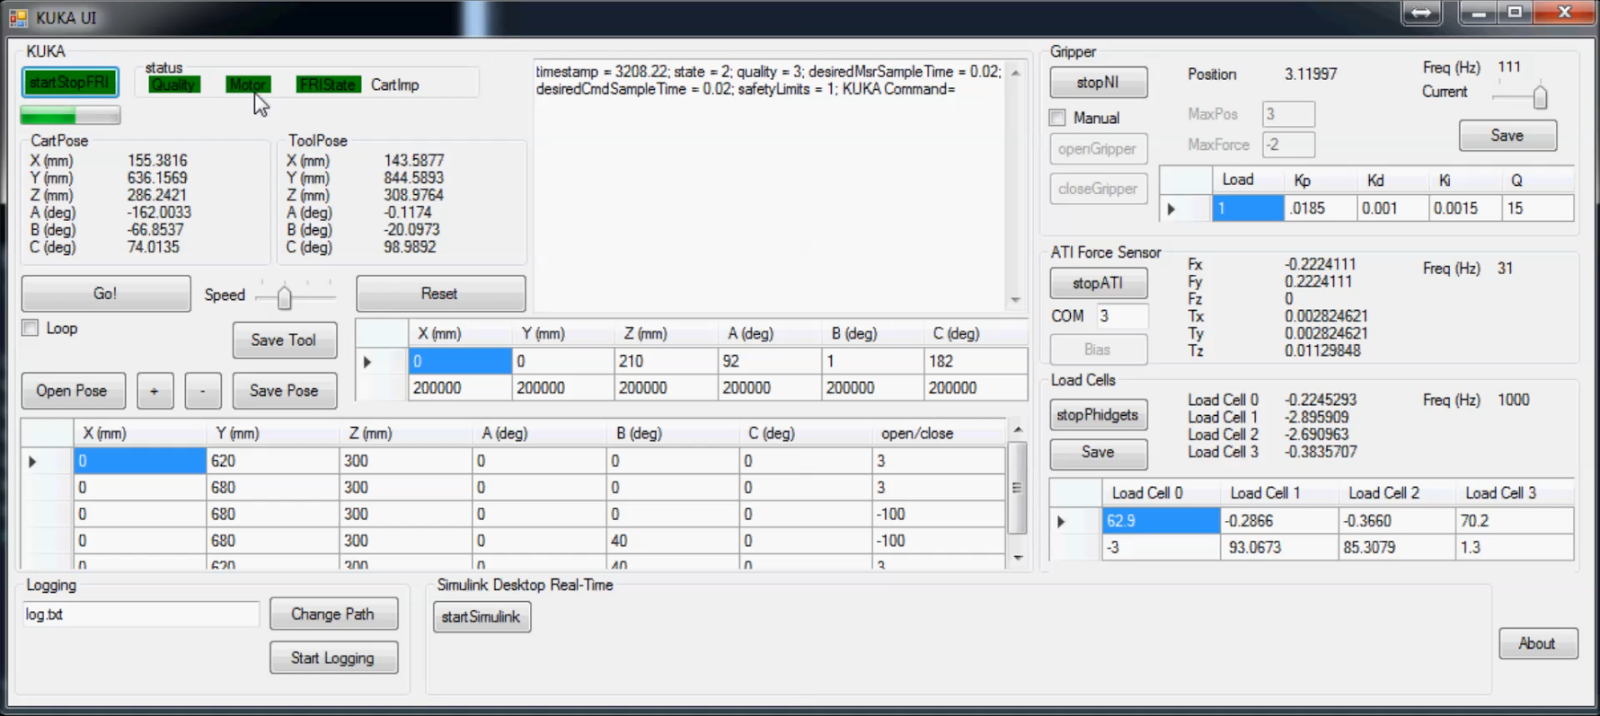
\includegraphics[width=0.99\linewidth]{figures/kuka-interface2}
	\caption{KUKA Robotics graphical user interface (\cite{abdeetedal2017kuka})}
	\label{fig:Kuka}
\end{figure} 
\begin{figure}[!h]
	\centering
	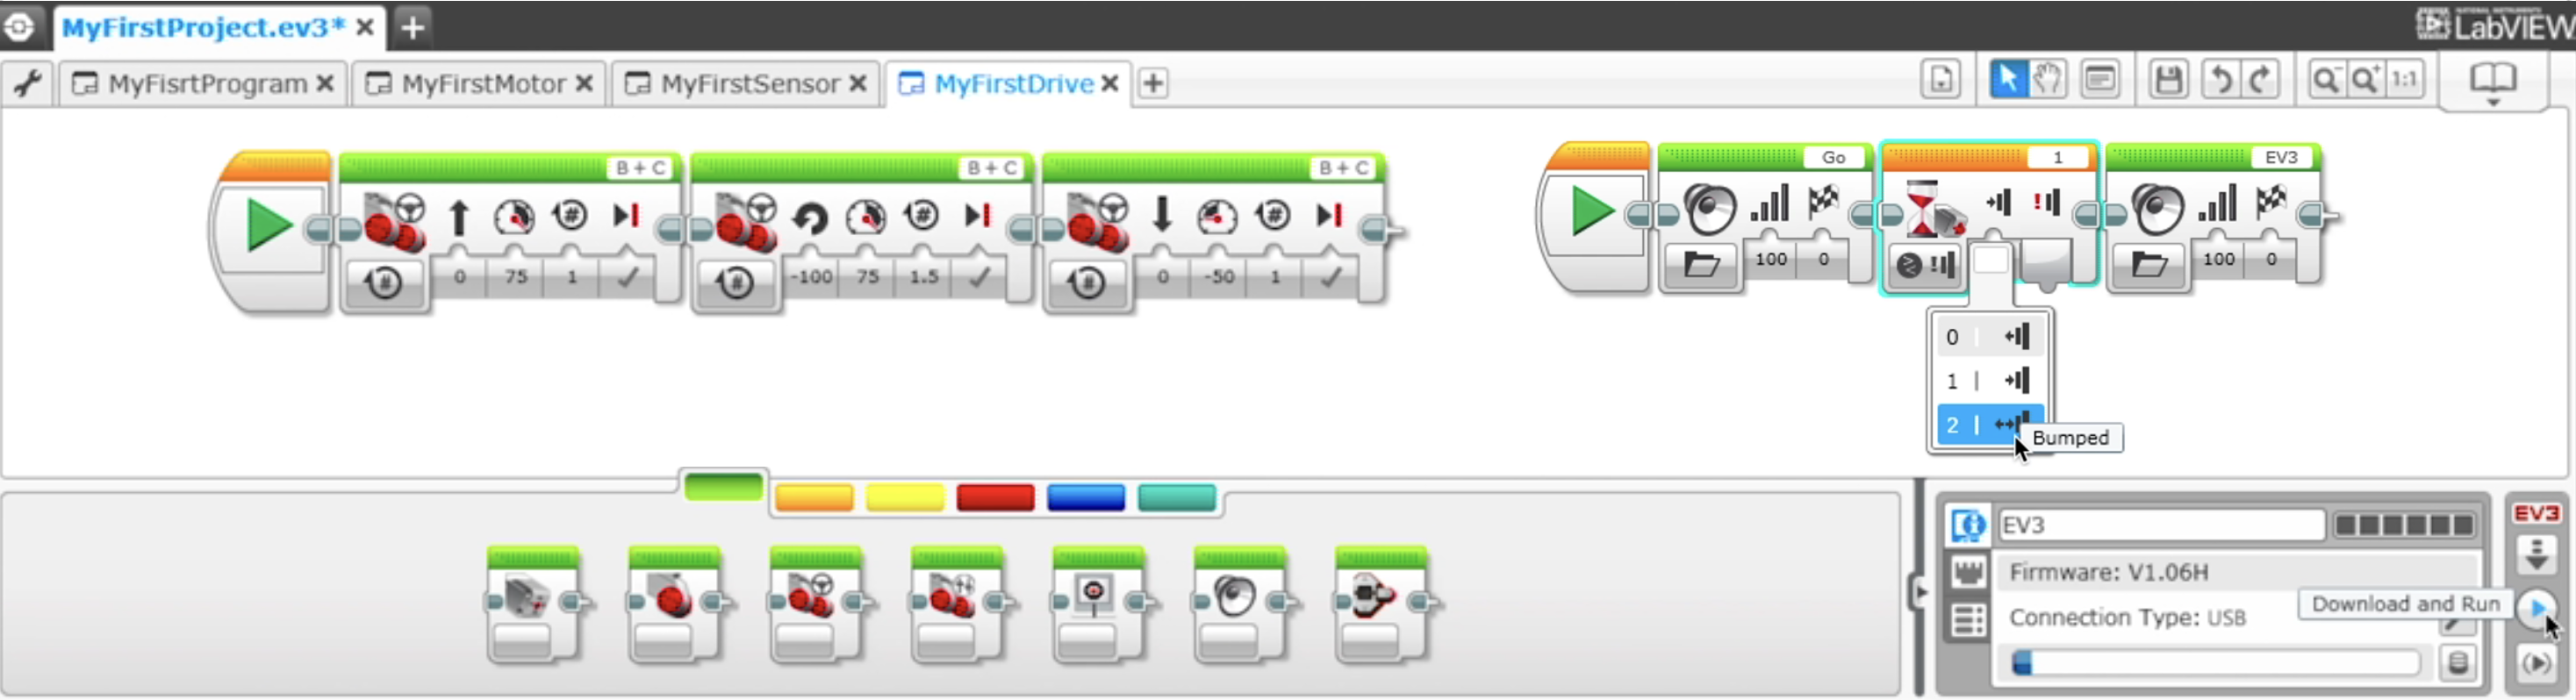
\includegraphics[width=0.94\linewidth]{figures/lego-mindstorm2}
	\caption{Lego Mindstorms EV3 icon-based interface (\cite{lego2003})}
	\label{fig:lego-mindstorm}
\end{figure} 
\begin{figure}[!h]
	\centering
	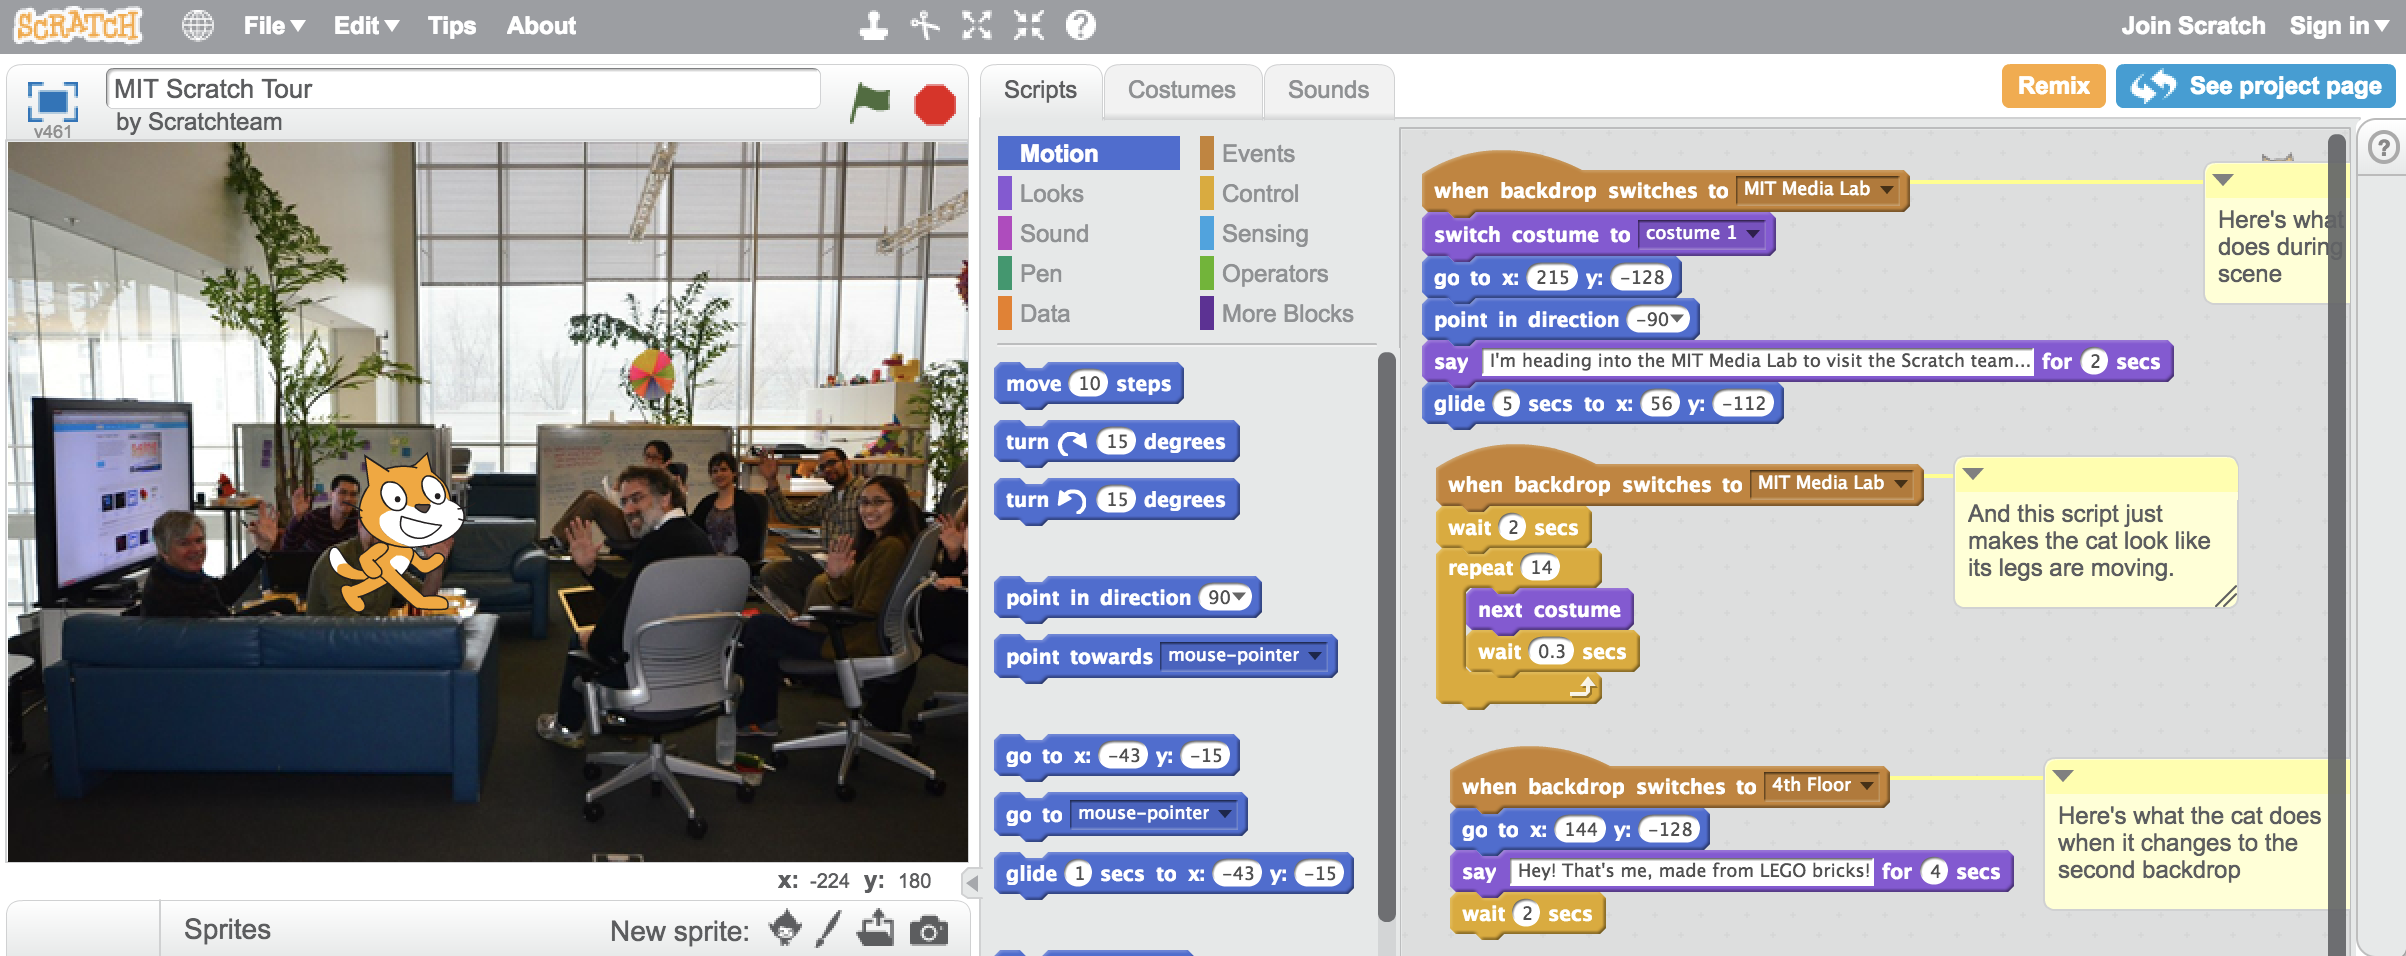
\includegraphics[width=0.94\linewidth]{figures/scratch-interface}
	\caption{Scratch: block-based visual programming language (\cite{majed2014learn})}
	\label{fig:scratch-interface}
\end{figure} 

\subsection{Policy derivation techniques}
\subsubsection{Low-level skill learning}\label{ssec:lowlevel}
Low-level representations focus on learning action trajectories or motions that can be generalised and applied to different tasks.
In the literature low-level actions have been referred to as \textit{skill, motor skill, primitive action,} or \textit{low-level motion} (\cite{chernova2014robot}).
Low-level actions can be learned from trajectory demonstrations using Gaussian Mixture Models (\cite{billard2008robot}) or Dynamic Movement Primitives (\cite{pastor2009learning}).
They can also be learned from keyframe-based demonstrations, %which consist of differential equations that can create a smooth trajectory sto a new goal point.
where the user kinesthetically manipulates the robot's arm to record a series of end-effector poses, referred to as \textit{keyframes} (\cite{akgun2012keyframe}). 
Actions are represented as a sparse sequence of gripper states (open/close) and end-effector poses relative to perceived objects or to the robot's coordinate frame.
\cite{akgun2012keyframe} compares techniques to learn from trajectory with keyframe-based demonstrations and propose learning from hybrid demonstrations that is suitable for learning any type of skill (\fig{fig:lowlevel}).
\cite{alexandrova2014robot} implemented an end-user robot programming system to teach generalisable actions from a single demonstration where keyframes are automatically inferred and actions can be modified retrospectively via a graphical user interface (\fig{fig:alexandrova-gui}).
%An end-effector pose can be relative to the robot's base or to a landmark previously detected by the robot.
%Landmarks are only known to the robot after a table top detection step has been performed.

\begin{figure}[!h]
	\centering
	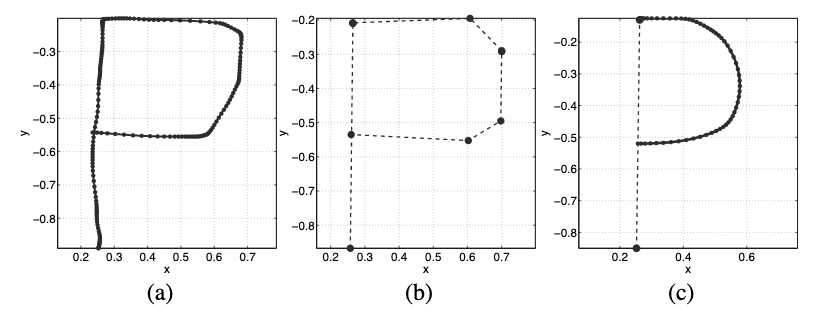
\includegraphics[width=0.7\linewidth]{figures/kLfd}
	\caption{Sample demonstrations of the letter P in 2D: (a) trajectory demonstration (b) keyframe-based demonstration (c) hybrid demonstration (\cite{akgun2012keyframe}).}
	\label{fig:lowlevel}
\end{figure} 

\begin{figure}[!h]
	\centering
	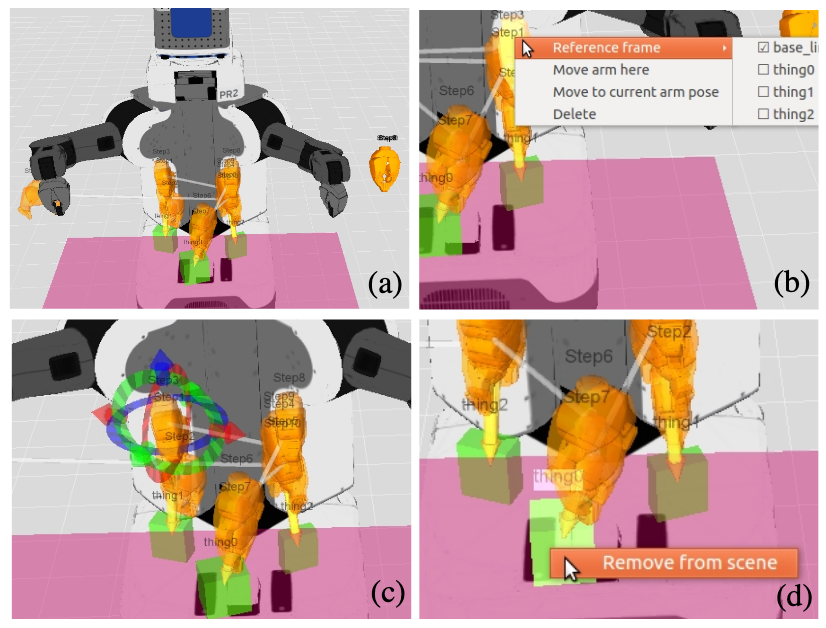
\includegraphics[width=0.7\linewidth]{figures/alexandrova-gui}
	\caption{Robot programming by keyframe-based demonstration using a graphical user interface that allows retrospectively editing (\cite{alexandrova2014robot})}
	\label{fig:alexandrova-gui}
\end{figure} 

\subsubsection{High-level task learning}\label{ssec:highlevel}
High-level task learning focuses on learning the \textit{sequence} of primitive actions, \ie the order to execute them.
Primitive actions are generally preprogrammed into the robot (\cite{peppoloni2014ros}), where high-level tasks are learned from observing complete task executions and extracting the primitive actions.
\citet{paxton2017costar} represent task plans with Behaviour Trees that users can modify manually to adapt to other tasks.
%For learning high-level tasks it is assumed that a set of low-level primitive actions is . 
\cite{she2014teaching} teaches the robot new high-level tasks by instructing the robot a sequence of lower-level actions.
Rather than representing the new action as an action sequence, it is modelled by their desired goal states obtained from object states at the beginning and at the end of the instruction.
% calculated as: $A_i(c_1 \dots c_k) = (S_e - S_e \cap S_b) \cup p_{grip}$ where $c_i$ are objects in the scene, $S_b$ and $S_e$ are the states at the beginning and end of the instruction and $p_{grip} = \{open, close\}$ is the gripper status at the end of instruction.
\cite{ahmadzadeh2015learning} learns the task goal by inferring preconditions and effects from multiple demonstrations.
%As the work uses the blocks world domain with a single object type (`block'), an operator for the new high-level action can be inferred easily. 
%Preconditions and effects for the domain are already specified in advance.

\subsection{Learning from data} \label{subsec:Gathering data}
There are different ways to learn from data depending on the amount provided at a time (incremental vs batch learning) and the type of data.
The robot can learn from data that is directly related to the desired behaviour and has been selected by a teacher (\eg from optimal teacher demonstrations), which we refer to as learning from \textit{biased} data.
If the robot learns from data that is not directly related to its executed behaviour (\eg from trial and error), we refer to it as learning from \textit{unbiased} data.
Thus, we differentiate automatic programming systems between Machine Learning (\sect{sssec:Learning Systems}), where the robot learns from \textit{unbiased} data, and Programming by Demonstration (\sect{sssec:PbD}), where the robot learns from \textit{biased} data.
In Machine Learning, the data can be provided directly to the robot (\eg Deep Learning) or acquired by self-exploration of the environment (\eg Reinforcement Learning).
Recent approaches have combined multiple techniques to improve the performance and accelerate the learning process, \eg Deep Reinforcement Learning (\cite{arulkumaran2017brief}) or PbD for Reinforcement Learning (\cite{hester2017learning}).
As this is beyond the scope of this thesis, we will give a brief overview of the main techniques and leave their discussion for future work.


\subsection{Machine Learning Systems}\label{sssec:Learning Systems}
Machine Learning (ML) systems use inductive inference to learn a policy from unbiased data, which includes data unrelated to the desired robot behaviour.
%It usually consists of video images (\cite{yang2016development}) or simulated executions (\cite{bibid}).
% by taking examples provided by the user or from self-exploration of the robot. 
The goal of these systems is to construct programs that allow the robot to automatically improve its performance with increasing amounts of data. 
Even though ML algorithms have been around since the 1980s, it has only become popular in the past few decades. 
The rise of the internet led to Big Data, improved knowledge sharing, and advances in techniques to process and store data efficiently triggered a wave of new ML techniques.
%Developments in various research areas such as computer vision have impacted the field of robotics.
Recent applications of ML in robotics (\cite{mlrobotics}) include research areas such as Computer Vision (or Robot Vision) for the identification and sorting of objects (\cite{stager2013computer}) and Imitation Learning to learn action plans from watching unconstrained videos (\cite{Yang2015}).
Many approaches derive a policy using vision by having the robot learn from image or video data or by observing a human teacher (\cite{kuniyoshi1994learning}).

We differentiate between the provided input data (\fig{fig:ml-types}): 
In Deep Learning (DL) (\cite{schmidhuber2015deep}), data is provided directly to the robot in either labelled (Supervised learning) or unlabelled format (Unsupervised learning).
DL systems generally use artificial Neural Networks (NN) which require large amounts of data and computation power to learn the desired behaviour.
Techniques are divided into supervised (\eg Classification, Regression) and unsupervised (\eg Clustering) learning, using labelled and unlabelled data respectively.
%\cite{billard2001robust} used NN to learn the motion of a human arm in 3D.

In Reinforcement Learning (RL)  (\cite{sutton1998reinforcement,kaelbling1996reinforcement,gosavi2009reinforcement}) the robot acquires data autonomously by exploring its environment.
The robot enters different states depending on the actions it takes and learns from the observed state changes.
While taking random actions, the robot uses a reward function to learn its policy and refines it by updating expected rewards with observed outcomes.
However, setting up the system's states, actions and initial policy is often difficult and usually requires robotics experts.
\cite{kober2013reinforcement} provides a survey of RL techniques to generate robot behaviours and highlights the main challenges that are faced.
Since the robot has to explore many states before it can learn the correct behaviour, RL systems usually take hundred or thousands of training examples which are usually collected in a simulated environment.
To accelerate the learning and reduce the amount of exploration required, recent work includes teacher demonstrations with RL solutions (\cite{martinez2017relational,hester2017learning}).


%There are two main classes of RL approaches, namely \textit{model-based} (\cite{polydoros2017survey}) and \textit{model-free }(\cite{kober2013reinforcement}) methods, differentiating between whether a model of the interactions between the robot and the environment is used, or whether it learns from samples.
%While model-based methods converge faster to the optimal solution, an accurate model is not always available and can impact the learning process.
%Model-free methods require the robot to learn from samples, resulting in a slow convergence to the optimal solution.

%In real world scenarios robots require teacher input to learn behaviours efficiently. 
%\todo{Similar to our work: \cite{martinez2017relational}}

%Inverse reinforcement learning (\cite{abbeel2011inverse}) is a supervised RL mode where the learner tries to acquire the reward function from demonstrated behaviours.
%This is can also be considered a learning from demonstration approach.

\begin{figure}[ht]
	\centering
	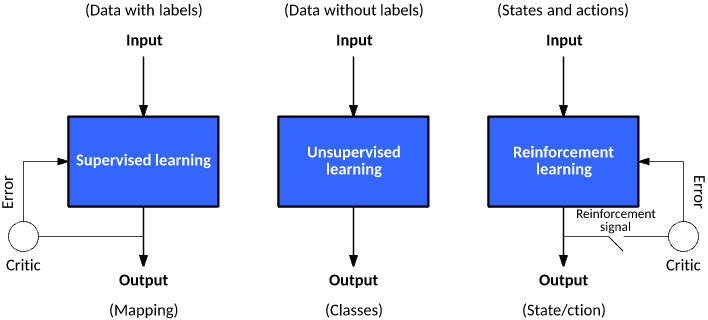
\includegraphics[width=\linewidth]{figures/ml-techniques}
	\caption{Types of Machine learning: Deep learning (supervised and unsupervised learning) and Reinforcement learning (\cite{jones2017models})}
	\label{fig:ml-types}
\end{figure}

\subsection{Programming by Demonstration}\label{sssec:PbD}
Programming by Demonstration (PbD) (\cite{billard2016learning,argall2009survey}) describes various techniques where the robot learns new behaviours from teacher demonstrations.
In the literature, it has also been referred to as \textit{Learning from Demonstration, Imitation Learning, Learning by Showing, Learning from Observation, Behavioral Cloning or Mimicry}.
It provides an intuitive medium to allow non-roboticists to communicate skills to robots without having to write code.
Unlike ML solutions, the provided data is biased, \ie directly correlated with the robots executed behaviour (\eg human teachers providing optimal demonstrations).
The underlying concept is for the robot to learn a new skill more efficiently from these selected demonstrations, thus reducing the complexity of the search space and accelerating learning.
As the teacher selectively provides demonstrations that the robot should learn from, the data is generally sparse and research has focused on learning from as few demonstrations as possible.
%%%%% Gathering demonstrations
The user can choose to provide positive or negative examples (\cite{grollman2012robot}). %, to allow the robot to learn more efficiently by reducing the search space for possible solutions.
Positive examples are demonstration data showing what the robot should do and what it can learn directly from. %, \ie where an action changes predicates.
Negative examples are what the robot should \textit{avoid} and help to generalise faster by eliminating bad solutions from the search space. %, \ie when an action fails because its preconditions are not satisfied.
\cite{walsh2010efficient} noted that negative examples are highly uninformative as the learner cannot easily determine the reason for the failure, while positive examples provide very useful information as a superset of the literals that belong to the action preconditions is identified.

There are different techniques to learn a policy depending on how demonstrations are provided to the robot and the chosen interaction modalities.
The robot can learn from simply observing the teacher demonstration (Learning by Observation).%, similar to Deep Learning techniques where the robot is provided with large amounts of data to learn from (\cite{kuniyoshi1994learning,yang2016development}).
%While Learning by exploration allows the robot to refine the policy on its own, it can be combined with teacher critique to accelerate learning. 
As human demonstrations are often noisy or suboptimal, interactive policy refinement techniques can be used, where robots learn from continuous feedback provided by the teacher (Active or Interactive Learning).
%In the following sections we will discuss these approaches.

%``Programming by demonstration (PbD) has become a central topic of robotics and spans across general research areas such as human-robot interaction, machine learning, machine vision and motor control" (\cite{billard2008robot}).

%PbD systems have been used in the industry for creating assembly programs. 
%It offers a framework for service robotics applications, independent of the robot platform, and reduces the overhead of reprogramming the robot for different tasks.
%In recent years there has been significant work in PbD to move from pure imitation to intelligent systems that learn flexible task executions. 
%PbD systems may learn task descriptions from interpreted data to adapt the learned task to changing environments.

\subsubsection{Providing demonstrations}
There exist various techniques for providing demonstrations.
\cite{argall2009survey} define four categories by differentiating between the choice of the demonstrator (human or robot) and who executes the demonstration:
The teacher could demonstrate either using their own hands (\textit{shadowing} %TODO; add references
 or \textit{external observation}), by wearing sensors (\textit{sensors on teacher}), or by moving the robot's joints directly (\textit{kinesthetic teaching} or \textit{teleoperation}).
If the demonstration is not recorded directly on the robot's joints (\eg shadowing), the demonstrated trajectory has to be extracted and mapped to the robot's joints.
This is related to the correspondence problem (\cite{nehaniv2002correspondence}), which describes the difference of humans and robots regarding their sensing abilities and physical embodiment.
If the robot joints are recorded directly from the demonstration (\eg kinesthetic teaching), this problem is eliminated.
Previous work showed that kinesthetic guidance can be problematic in narrow spaces (\cite{wrede2013user}) or if the objects are large or dangerous to operate (\cite{chernova2014robot}).
However, comparing kinesthetic teaching with teleoperation showed that kinesthetic teaching produced better results in terms of efficiency, effectiveness (success and error rate), and usability (\cite{fischer2016comparison,chernova2014robot,akgun2011robot}).


\subsubsection{Interaction modalities}
There are different ways for the teacher to transfer the data to the robot, for example using voice, vision, touch or gestures.
PbD systems often use touch to provide demonstrations, \ie by kinesthetically moving the robot's joints.
%Demonstrations can also be provided by kinesthetically moving the robot's joints, allowing the robot to go through the action execution.
%Natural language is the most intuitive way for humans to communicate instructions but may need some form of clarification and learning system in order to work efficiently. 
Voice recognition can be used during demonstrations to activate in-built actions such as opening gripper or saving end-effector poses (\cite{alexandrova2014robot}).
Such instructive systems provide the user with a high-level control to program the action sequence by commanding sub-actions that have already been programmed into the robot (\cite{forbes2015robot}).
%The teacher can also demonstrate the action using their own hands, while the robot observes the motion (\cite{kuniyoshi1994learning}).
%Gestures can be used to direct the attention of the robot for indicating objects in a scene to which the instructions apply. % TODO(\cite{bibid}).
Multi-modal communication that combines information from vision, gesture and voice sources can be used to clarify instructions to the robot, for example mentioning `that table' and gesturing the relevant object at the same time. % (\cite{bibid}).
\cite{profanter2015analysis} evaluated four input modalities (touch, gesture, speech, 3D tracking device) and showed that users preferred touch and gesture input, while speech input was the least preferred modality.

%Instructive systems use voice recognition to command robots to carry out tasks while performing a demonstration.

%Programming by demonstration is an approach to learn this policy from demonstration data, known as \textit{examples}.
% ``Examples are sequences of state-action pairs that are recorded during the teacher's demonstration of the desired robot behaviour." \cite{argall2009survey} 
%Unlike learning techniques in reinforcement learning, PbD is aimed at learning from correct examples only.
%Thus, PbD can be seen as a subset of Supervised Learning, as the agent is presented with labelled training data and tries to learn an approximation of the function, which produced the data (\cite{argall2009survey}).


%In contrast to reinforcement learning techniques, where the policy is learned from arbitrarily positive and negative experience, PbD approaches derive the policy from a dataset of selected examples.
%The robot derives a policy in various ways (\sect{subsec:Deriving a policy}). 

\subsubsection{Interactive policy refinement techniques}\label{subsec:Other RP Methods}
%\subsubsection{Learning by Exploration}\label{sssec:LbExploration}
%- the robot acquires data from interaction with its environment
%- need a reward function which allows him to learn from the data
%1. Reinforcement learning (\cite{sutton1998reinforcement}, \cite{mnih2015human})
% - reward function can be specified by the user, robot learns policy by self-exploration
% 2. Inverse reinforcement learning (\cite{abbeel2004apprenticeship})
% - robot is given teacher demonstrations and learns reward function
For active, or \textit{interactive}, learning, the teacher is involved in the learning process by providing regular feedback to the learned action  %provides the robot with initial data, observes its performance when executing the learned action and then provides further feedback 
(\cite{nicolescu2003natural,calinon2007active,calinon2007incremental}).
%They implement systems, which actively involve the teacher in the robot's learning process, by providing human guidance to a humanoid robot. 
The robot first observes the demonstration performed by the teacher. 
When it reproduces the action, the teacher can improve and correct the movement by physically moving its limbs.
In \cite{nicolescu2003natural} the robot refines the learned skill using feedback cues provided by the teacher and by inserting or removing behaviours from the network of abstract behaviours.
Learning tasks from interactions with a teacher is also known as \textit{Interactive Task Learning} (\cite{laird2017interactive}), where the goal is to learn through natural communication and to improve performance via instruction, demonstration, and feedback. 
The robot can also request feedback from the teacher when encountering problems during action execution (\cite{cakmak2012aaai,abdo2013learning,martinez2017relational}).
Other policy refinement approaches allow the teacher to modify the taught actions using a graphical interface, therefore minimising the number of demonstrations required.
 (\cite{alexandrova2015roboflow,perzylo2016intuitive,paxton2017costar,stenmark2017simplified}).

%\cite{martinez2017relational} propose a relational RL solution with guided demonstrations where the robot requests for help from the human teacher to reduce the learning time.
%However, demonstrations are only requested if they yield significant improvements as the teacher's time is considered more valuable than the robot's time.

%ITL: The central challenge consists of ``converting externally specified descriptions of a task into internal representations that are incrementally integrated with existing knowledge".
%The authors mention that PbD simplifies the programming process but is generally limited by the types of tasks being taught due to the restricted knowledge that can be transferred through demonstrations.

%\todo{check Imitation learning survey}

%\subsubsection{Robot feedback}
%Robot feedback is important to provide the teacher with enough information about what to demonstrate to the robot.
%Reasons such as wrong preconditions or missing action effects can lead to failures.
%Failures can be explained using excuses \cite{?}
%Benchmark: \cite{martinez2017relational} uses 3 examples from Planning competitions

\section{End-user Involvement}\label{sssec:End-User Involvement}
There are different levels of end-user involvement in robot programming, such as writing and organising the execution code in manual programming or providing data in the form of demonstrations, labelled or unlabelled data for automatic programming systems. %biased or unbiased data, and defining reward functions. 
Inspired by \cite{kormushev2013reinforcement} who compared different robot teaching approaches,
%by computational complexity with difficulty for the teacher.
Table \ref{tab:enduserinvolvement} compares the presented robot programming approaches by user involvement task, expertise required, as well as data and time required to learn a skill.
For the last three categories, we assign a ranking from `high', `moderately high', to `moderately low' and `low'.
The required expertise corresponds to how hard it is for an end-user without programming experience to complete the user tasks for the programming approach.
%In this case we consider experts as users who have received formal training or experience in the stated robot programming method, \eg programming languages or RL/DL-related concepts.

While manual programming approaches do not require any data, they can be considered most difficult and time consuming, as the user has to write or sequence the execution code manually.
Even though visual programming facilitates the programming experience over text-based programming, it still requires users to have a good understanding of the constructed program flow.

Programming by demonstration (PbD) provides a more intuitive low-effort solution, where the teacher's main task involves providing demonstrations to the robot.
Since PbD solutions allow the robot to learn from a sparse set of examples, the data and time required to learn a skill is moderately low.
While it does not require programming experts, the difficulty lies in providing correct examples that are diverse enough to allow the robot to learn a generalised skill that is applicable to new scenarios.

Other automated programming approaches, such as Reinforcement Learning (RL) and Deep Learning (DL), allow the robot to learn autonomously, but require programming and domain experts to prepare the system input (\eg label or preprocess data for DL, define policy and reward functions for RL). %, resulting in a rather high difficulty for the teacher.
These systems generally require vast amounts of data and computation power to learn a skill and are usually trained in simulation.
%If the labelled data is available online, users are left with tuning the system parameters to avoid overfitting.
%The end-users that use these approaches are generally domain experts who have the required programming experience to complete the involved tasks.


%\begin{figure}[ht]
%	\centering
%	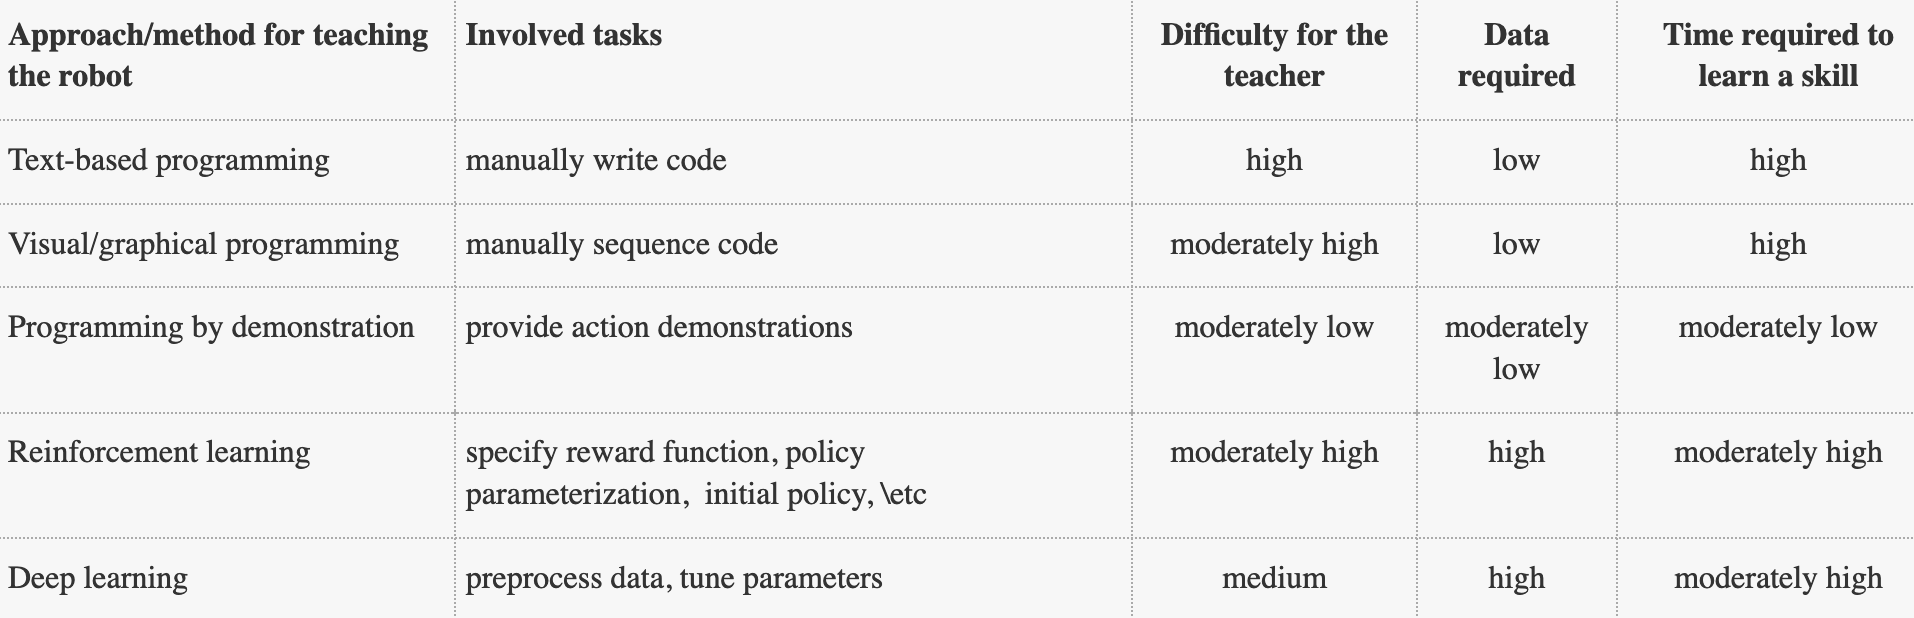
\includegraphics[width=\linewidth]{figures/robot-programming-comparison}
%	\caption{End-user involvement for common robot programming approaches}
%	\label{tab:enduserinvolvement}
%\end{figure}

\begin{table}[h]
	\centering
	\caption{End-user involvement for common robot programming approaches}
	\label{tab:enduserinvolvement}
	\begin{tabular}{@{}l@{\hskip1.5pt}l@{\hskip1pt}c@{\hskip1pt}c@{\hskip1pt}c}
		\noindent\begin{tabular}{@{}l}
			\textbf{Programming}\\
			\textbf{approach}
		\end{tabular} & \textbf{Involved tasks}& 
		\begin{tabular}{c}
			\textbf{Expertise}\\
			\textbf{required}
		\end{tabular} & 
		\begin{tabular}{c}
			\textbf{Data}\\
			\textbf{required}
		\end{tabular} &
		 \begin{tabular}{c}
			\textbf{Time required}\\
			\textbf{to learn skill}
		\end{tabular} \\ \hline
		Text-based  & manually write code  & high& - & high\\ \hline
		Visual/graphical & manually sequence code & 
		\noindent\begin{tabular}{@{}c}
			{moderately}\\
			{high}
		\end{tabular}  & - & high\\ \hline
		\noindent\begin{tabular}{@{}l}
			{Programming}\\
			{by demonstration}
		\end{tabular} & provide demonstrations & 
		\noindent\begin{tabular}{@{}c}
		{moderately}\\
		{low}
		\end{tabular} & 
			\noindent\begin{tabular}{@{}c}
			{moderately}\\
			{low}
		\end{tabular}  & 
			\noindent\begin{tabular}{@{}c}
			{moderately}\\
			{low}
		\end{tabular}   \\ \hline
		\noindent\begin{tabular}{@{}l}
			{Reinforcement}\\
			{learning}
		\end{tabular} &
		\noindent\begin{tabular}{@{}l}
			specify reward function, \\
			policy parameterization, \\
			initial policy, \etc \\
		\end{tabular} 
		& 
		\noindent\begin{tabular}{@{}c}
			{moderately}\\
			{high}
		\end{tabular} & high & 
		\noindent\begin{tabular}{@{}c}
			{moderately}\\
			{high}
		\end{tabular}  \\ \hline
		Deep learning  & 
		\noindent\begin{tabular}{@{}l}
			preprocess data,\\ 
			tune parameters \\
		\end{tabular}  & 
		\noindent\begin{tabular}{@{}c}
		{moderately}\\
		{high}
	\end{tabular} & high& 
	\noindent\begin{tabular}{@{}c}
	{moderately}\\
	{high}
\end{tabular} 
	\end{tabular}
\end{table}
%
%\begin{table}[h]
%	\centering
%	\begin{tabular}{llcc}
%		 \textbf{Programming method} & \begin{tabular}{@{}l@{}}\textbf{End-user task} \\ \textbf{required}\end{tabular} & \begin{tabular}{@{}l@{}}\textbf{Effort} \\ \textbf{required}\end{tabular} & \begin{tabular}{@{}l@{}}\textbf{Expertise} \\ \textbf{required}\end{tabular} \\ \hline
%		Write code manually & Text-based programming & high & yes \\
%		Organise code sequence & Visual programming & moderately high & no \\
%		\begin{tabular}{@{}l@{}}Provide complete data, \\ Tune parameters \end{tabular} & Deep learning (DL) & moderate & yes \\
%		Provide partial data & \begin{tabular}{@{}l@{}}Programming by \\ demonstration (PbD)\end{tabular}
%		 & moderately low & no \\
%		Define reward function & Reinforcement learning (RL) & moderately low & yes 
%	\end{tabular}
%\caption{End-user involvement for common robot programming approaches}
%\label{tab:enduserinvolvement}
%\end{table}



%\section{Robot Programming in Industrial Environments}\label{subsec:RP in Industrial Enviroments}
%The deployment of robots in industrial environments introduces additional constraints to the robot programming process, such as limited resources, time constraints, limited programming expertise, product-specific tasks.
%\cite{pan2012recent} give an overview of three main robot programming methods for industrial robots: offline programming, online programming, and using Augmented Reality. 
%
%\subsection{Offline Programming}\label{sssec:Offline Programming}
%Offline Programming (OLP) is based on 3D CAD data that models the complete robot work cell and lets the user fine-tune the properties of the robot's movements before generating a program that can be downloaded to the robot. 
%It is more efficient when programming complex systems with large volumes and more reliable compared to online programming. 
%As it requires a great amount of programming effort and a long delivery time, it requires high programming overhead and is not efficient for the development of smaller product volumes or customised software.
%
%Robot designers and users have developed computational platforms for OLP systems in form of packages that allow secondary development for specific applications. 
%These OLP packages simulate not only robot trajectories and assembly tasks, but can also model interactions of several manufacturing processes, resources and product maintenance issues. 
%Almost every robot manufacturer has its own OLP software. 
%There exist also generic OLP software that are more flexible for hardware from different manufacturers.
%
%Current OLP systems do not provide functions for the complete OLP process but include steps that need to be created manually. 
%Due to the high costs of OLP systems, their use is not cost-efficient for small to medium-sized enterprises.
%
%\subsection{Online Programming}\label{sssec:Online Programming}
%In online programming methods the robot program commands the robot to move through a recorded sequence of end-effector postures which form a complete task. 
%The postures are recorded using the teach pendant to manually move the end-effector to the desired position and orientation of the task. 
%Due to its simplicity, intuitiveness, and low programming skill requirement, this method is widely used. 
%However, it is only suitable for programming applications with uncomplicated processes and work pieces with simple geometry. 
%Once the program has been generated, it is difficult to make further amendments.
%
%\subsection{Augmented Reality}\label{sssec:Augmented Reality}
%The use of augmented reality (AR) is a revolutionary concept where computer-generated 3D objects are blended onto a real world scene to enhance the user's interaction with the real world (\cite{pettersen2003augmented}). 
%Robot programming using AR allows offline programming to be performed without the need to model the workpiece in the virtual environment (\cite{pan2012recent}). 
%It can eliminate technical difficulties faced by OLP techniques such as the calibration between the virtual and the real world.


